\documentclass[a4paper]{article}
\usepackage[a4paper,margin=0mm]{geometry}
\usepackage{fontspec}
\usepackage{unicode-math}
\usepackage{tikz}
\usetikzlibrary{fit,calc,positioning}
\usepackage[table]{xcolor}
\usepackage[absolute]{textpos}
\usepackage{array}

\setmainfont{Libertinus Serif}
\setsansfont{Libertinus Sans}
\setmathfont{Libertinus Math}

\definecolor{accent}{HTML}{F46530}
\definecolor{badge}{HTML}{FFBDA5}
\definecolor{ink}{HTML}{2A2E30}

\setlength{\TPHorizModule}{1mm}
\setlength{\TPVertModule}{1mm}
\setlength{\parindent}{0pt}
\pagestyle{empty}

\newcommand{\topicheader}[2]{%
\begin{textblock*}{194mm}(16mm,10mm)
\begin{tikzpicture}
\node[fill=accent,text=white,font=\sffamily\bfseries\fontsize{13}{13}\selectfont,
      minimum width=9mm,minimum height=9mm,inner sep=0pt] at (4.5mm,-4.5mm) {#1};
\node[font=\sffamily\bfseries\fontsize{15}{16}\selectfont,text=ink,anchor=west] at (12mm,-4.5mm) {#2};
\end{tikzpicture}
\end{textblock*}
\begin{textblock*}{194mm}(16mm,22.5mm)

\begin{tikzpicture}
\fill[accent] (0,0) rectangle (194mm,0.5mm);
\end{tikzpicture}
\end{textblock*}
}

\newcommand{\pagekicker}[1]{%
\begin{textblock*}{100mm}(16mm,25.5mm)
\begin{tikzpicture}
\node[fill=ink,text=white,font=\sffamily\bfseries\fontsize{8}{8}\selectfont,
      inner sep=2.2pt,rounded corners=1pt] {\MakeUppercase{#1}};
\end{tikzpicture}
\end{textblock*}
}

\newcommand{\pagefooter}[1]{%
\begin{textblock*}{194mm}(8mm,286.41mm)
  
\begin{tikzpicture}
    \fill[accent] (0,0) rectangle (194mm,0.6mm);
  \end{tikzpicture}
\end{textblock*}
\begin{textblock*}{63.59mm}(8mm,288.27mm)
  {\sffamily\bfseries\color{accent}\fontsize{13}{16}\selectfont SAT 1200+}
\end{textblock*}
\begin{textblock*}{10mm}(188mm,288.27mm)
  \centering{\sffamily\color{accent}\fontsize{14}{16}\selectfont #1}
\end{textblock*}
}

\newcommand{\cardbg}[4]{%
\begin{textblock*}{#3mm}(#1mm,#2mm)
\begin{tikzpicture}
\fill[badge!22,rounded corners=3mm] (0,0) rectangle (#3mm,-#4mm);
\end{tikzpicture}
\end{textblock*}%
}

\newcommand{\pill}[3]{%
\begin{textblock*}{160mm}(#1mm,#2mm)
\begin{tikzpicture}
\node[fill=accent,text=white,anchor=north west,font=\sffamily\bfseries\fontsize{10}{10}\selectfont,
      rounded corners=8pt,inner xsep=5mm,inner ysep=1.8mm] at (0,0) {QOIDA ~\textperiodcentered~ #3};
\end{tikzpicture}
\end{textblock*}%
}

\arrayrulecolor{accent}
\setlength{\arrayrulewidth}{0.7pt}
\renewcommand{\arraystretch}{1.5}

\begin{document}

\topicheader{3}{O'nli kasrlar va foizlar}
\pagekicker{Formula sheet}
\pagefooter{19}
\mbox{}%

% ================= CARD 1: Vergul(nuqta)ni tekislash (y: 33-88) =================
\cardbg{16}{33}{178}{55}
\pill{26}{36}{Nuqtani tekislash}

\begin{textblock*}{70mm}(30mm,52mm)
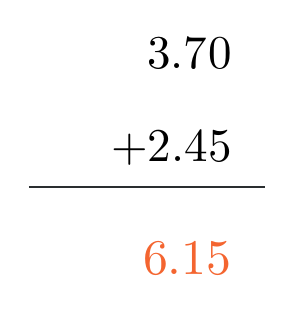
\begin{tikzpicture}[every node/.style={font=\fontsize{17}{17}\selectfont}]
\node[anchor=east] at (30mm,8mm) {$3.70$};
\node[anchor=east] at (30mm,-4mm) {$+2.45$};
\draw[ink,line width=0.8pt] (3mm,-9mm) -- (33mm,-9mm);
\node[anchor=east,text=accent,font=\sffamily\bfseries\fontsize{18}{18}\selectfont] at (30mm,-18mm) {$6.15$};
\end{tikzpicture}
\end{textblock*}

\begin{textblock*}{70mm}(112mm,58mm)
{\fontsize{10.5}{13}\selectfont\color{black!60}\itshape Qo'shish/ayirishdan oldin nuqtalarni ustma-ust tekislang; yetishmagan xonani nol bilan to'ldiring.}
\end{textblock*}

% ================= CARD 2: O'nli kasr <-> oddiy kasr (y: 94-149) =================
\cardbg{16}{94}{178}{55}
\pill{26}{97}{O'nli kasr $\leftrightarrow$ oddiy kasr}

\begin{textblock*}{158mm}(26mm,112mm)
\begin{tikzpicture}[every node/.style={font=\fontsize{14}{14}\selectfont}]
\node[anchor=west] at (0,0) {$0.75$};
\node[anchor=west,font=\fontsize{11}{11}\selectfont] at (18mm,0) {$=\dfrac{75}{100}$};
\node[anchor=west,text=accent,font=\sffamily\bfseries\fontsize{15}{15}\selectfont] at (48mm,0) {$=\dfrac{3}{4}$};
\node[anchor=west,font=\sffamily\scriptsize,text=black!55] at (68mm,1mm) {($\div25$, EKUB)};

\node[anchor=west] at (100mm,0) {$\dfrac{1}{8}$};
\node[anchor=west,font=\fontsize{13}{13}\selectfont] at (112mm,0) {$\xrightarrow{\ \div\ }$};
\node[anchor=west,text=accent,font=\sffamily\bfseries\fontsize{15}{15}\selectfont] at (132mm,0) {$0.125$};
\end{tikzpicture}
\end{textblock*}

\begin{textblock*}{158mm}(26mm,135mm)
{\fontsize{10.5}{13}\selectfont\color{black!60}\itshape Oxirgi xona qiymati maxrajni belgilaydi; teskarisida suratni maxrajga bo'ling.}
\end{textblock*}

% ================= CARD 3: Foiz <-> o'nli kasr (y: 155-210) =================
\cardbg{16}{155}{178}{55}
\pill{26}{158}{Foiz $\leftrightarrow$ o'nli kasr}

\begin{textblock*}{158mm}(26mm,174mm)

\begin{tikzpicture}[every node/.style={font=\fontsize{15}{15}\selectfont}]
\node[anchor=west] at (0,0) {$45\%$};
\node[anchor=west,font=\fontsize{12}{12}\selectfont] at (20mm,0) {$\xrightarrow{\ \div100\ }$};
\node[anchor=west,text=accent,font=\sffamily\bfseries\fontsize{16}{16}\selectfont] at (52mm,0) {$0.45$};

\node[anchor=west] at (95mm,0) {$0.6$};
\node[anchor=west,font=\fontsize{12}{12}\selectfont] at (112mm,0) {$\xrightarrow{\ \times100\ }$};
\node[anchor=west,text=accent,font=\sffamily\bfseries\fontsize{16}{16}\selectfont] at (144mm,0) {$60\%$};
\end{tikzpicture}
\end{textblock*}

\begin{textblock*}{158mm}(26mm,197mm)
{\fontsize{10.5}{13}\selectfont\color{black!60}\itshape Foizdan o'nli kasrga: vergulni 2 xona chapga suring. Teskarisida: 2 xona o'ngga.}
\end{textblock*}

% ================= CARD 4: Sonning foizi (y: 216-271) =================
\cardbg{16}{216}{178}{55}
\pill{26}{219}{Sonning foizi}

\begin{textblock*}{158mm}(26mm,235mm)
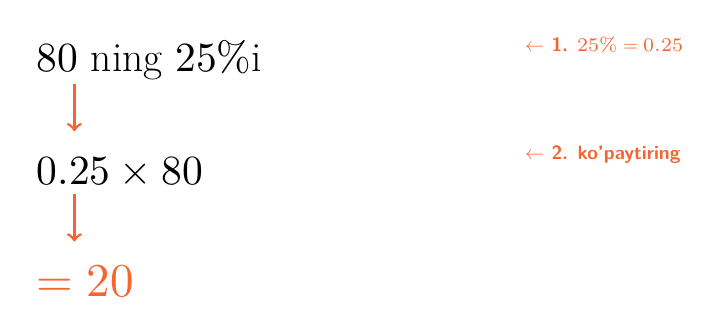
\begin{tikzpicture}[every node/.style={font=\fontsize{15}{15}\selectfont}]
\node[anchor=west] (l0) at (0,0) {$80 \text{ ning } 25\%\text{i}$};
\node[anchor=west,font=\sffamily\bfseries\scriptsize,text=accent] at (62mm,2mm) {$\leftarrow$ 1. $25\%=0.25$};

\node[anchor=west] (l1) at (0,-14mm) {$0.25\times80$};
\node[anchor=west,font=\sffamily\bfseries\scriptsize,text=accent] at (62mm,-12mm) {$\leftarrow$ 2. ko'paytiring};

\node[anchor=west,font=\sffamily\bfseries\fontsize{17}{17}\selectfont,text=accent] (l2) at (0,-28mm) {$=20$};

\foreach \y in {-3,-17}{
  \draw[accent,->,line width=1pt] (6mm,\y mm) -- (6mm,\y mm -6mm);
}
\end{tikzpicture}
\end{textblock*}

\end{document}
